\chapter{Computer Vision and Machine Learning}
Vision is one of our primary senses. Therefore, it is understandable that we seek methods for capturing, storing, analyzing, and processing this kind of data. Digital image processing is a vast area of different disciplines, ranging from low-level operations such as noise reduction, image sharpening, and contrast adjustment through mid-level operations like classification and segmentation to high-level operations which involve making higher sense of the images and resembling human visual perception and intelligence \cite{Gonzalez2018}. 

Computer Vision, a subfield of computer science and an extension of digital image processing focuses on using computers to extract meaningful knowledge from images in various ways, thereby emulating the capabilities of the human brain and visual cortex \cite{Gonzalez2018}. As part of machine learning and artificial intelligence, computer vision uses automation algorithms to analyze and process visual data, including 2D and 3D images as well as videos \cite{Szeliski2022, Atallah2020}.

Machine learning is a subset of artificial intelligence, which includes both statistical learning and deep learning algorithms to make intelligent decisions based on data. Modern computer vision primarily utilizes deep learning techniques, as illustrated in figure \ref{fig:ai-ml}. In classical programming, we are designing an explicit program that produces desired outputs for specific inputs. In machine learning, however, we let the machine design an appropriate program, given the specified set of inputs and outputs (labels) by analyzing the features and patterns of the input with relation to the output \cite{Alam2021}.

\begin{figure}[H]
\begin{centering}
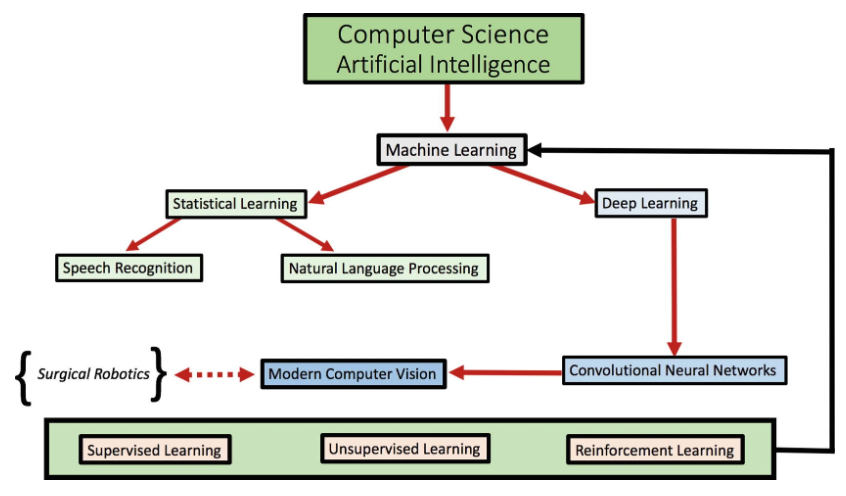
\includegraphics[width=12cm]{assets/images/aiml.png}
\par\end{centering}
\caption{Division of AI/ML \cite{Atallah2020}}
\label{fig:ai-ml}
\end{figure}

With the advent of deep learning \cite{LeCun2015} and especially convolutional neural networks \cite{Ronneberger2015}, computer vision is now a field of huge interest.

\section{Preprocessing}
Since the machine learning algorithms try to examine the relationship between input and output, we need to ensure an appropriate quality of the input data. Especially in medical imaging and digital histopathology, where the different staining techniques, scanning tools, or position of the tissue can vary widely and this can have an effect on the further analysis \cite{Hoque2024}.

In the domain of digital histopathology, a common issue are the varying intensities of purple, red, and pink tones of H\&E stained slides \cite{Hoque2024}. For this purpose, different stain normalization techniques were created. Among the examples, we can list the Macenko, Reinhart, or Zheng normalization techniques, which try to normalize the dataset of input images \cite{Hoque2024}. Among some other techniques, we can list the histogram equalization, Contrast-Limited Adaptive Histogram Equalization (CLAHE), and the power law (gamma) transformation \cite{Dabass2020}.

\section{Core Computer Vision Tasks}
When analyzing an image, we can come across the three main tasks \cite{Alam2021}. The example of each of these tasks can be seen in figure \ref{fig:aiml-tasks}.

\begin{figure}[H]
\begin{centering}
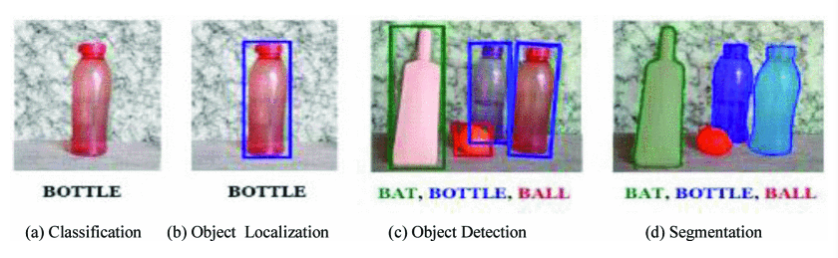
\includegraphics[width=12cm]{assets/images/aiml-tasks.png}
\par\end{centering}
\caption{Different Computer Vision tasks \cite{Alam2021}}
\label{fig:aiml-tasks}
\end{figure}

\subsection{Image Classification}
Image classification is used when we have a label categorizing the image into one of the classes (or multiple classes) in the set of classes \cite{Alam2021}. For example, in the medical imaging domain, we could label an image with the "disease" or "non-disease" class.

\subsection{Object Localization and Object Detection}
Object localization and object detection are very similar tasks. While the former is a task of localizing a single object instance in the image, the latter is a task where multiple instances of one or many objects should be detected and bounded \cite{Alam2021}.

\subsection{Segmentation} Sometimes we want to get a more detailed label than just an approximate object location (bounding rectangle). Segmentation utilizes pixel-level classification, where pixels can be labeled based on their relationship to various classes. According to \cite{Alam2021} we know two main types of segmentation:

\begin{itemize}
    \item Semantic segmentation, where each pixel of a certain class gets the same label, no matter the number of instances, and
    \item Instance segmentation, where the pixels of different instances of the same class are distinguished as well.
\end{itemize}

Apart from the currently most popular and interesting segmentation algorithms using deep learning, we also know some traditional segmentation techniques, like the GrabCut algorithm.

The GrabCut algorithm was first introduced in \cite{Rother2004} as a foreground extractor. With it, we are able to segment a foreground object and isolate it from the background. The GrabCut takes an image as an input, with a tight rectangular label indicating where the object we want to segment is located. Everything outside of this region is considered background and everything inside of this region is unknown. A user can hard-label parts of this region to explicitly indicate that those pixels belong to either foreground or background. Then a Gaussian Mixture Model models the the foreground and background regions. It utilizes color statistics to label unknown pixels as probable foreground or probable background. Next, a graph is created from these pixels, where each pixel represents a single node in the graph. In addition to pixel nodes, the source and the sink nodes are added to the graph. All foreground pixels are connected to the source node and similarly, all background pixels are connected to the sink node. The weights on the edges of the pixels that are connected both to the source and the sink node are defined by the probability of the pixel being either foreground or background. The edge information or the pixel similarity is used to define the weight on the edges between the pixels. Finally, a mincut algorithm processes the graph to separate the source and sink nodes. In the end, every pixel that is connected to the source node is labeled as foreground and every pixel connected to the sink node is labeled as background \cite{opencv_grabcut}.


\section{Learning Paradigms}
Computer vision algorithms can be further divided by how they can learn from the data \cite{Alam2021}.

\paragraph{Supervised Learning} In the supervised learning tasks, both the data and their respective labels are known and are available to the model during the training. Typical supervised learning tasks include classification, detection, and segmentation. By the quality and precision of the labels and the task goal, we can split supervised learning into three categories:

\begin{itemize}
    \item Standard supervised learning, when available labels are of the same quality as the labels we want to predict, e.g. bounding box to bounding box.
    \item Strong supervised learning, when the training labels contain richer information than the labels we want to predict, e.g. bounding box from pixel-level annotations.
    \item Weak supervised learning, when the training labels contain less precise information than the labels we want to predict, e.g. bounding box from image level annotation.
\end{itemize}

\paragraph{Unsupervised Learning} In unsupervised learning, on the other hand, the data labels are not available to the model during the training.
